\chapter{Algorytmy}
\label{cha:algorytmy}

W rozdziale tym omówione zostaną wybrane algorytmy śledzenia. Rozważona będzie również możliwość oraz skuteczność ich implementacji sprzętowej i sprzętowo-programowej.
%TODO reczej nie "my" .... unikamy takiej formy -zrobione.

\section{Śledzenie przez detekcję}
\label{sec:sledzenieprzezdetekcje}

Algorytm ten polega na detekcji obiektu i określeniu jego położenia (np. poprzez wyznaczenie środka ciężkości). Najważniejsze jest, by użyta metoda detekcji wykrywała obiekt zawsze, gdy ten znajduje się w kadrze.
%TODO można polemizować ... raczej należy mieć pewnonść co do detekcji, że zawsze, albo prawie zawsze zadziała. -coś zmieniłem, ale nie wiem czy teraz jest lepiej.
Należy zauważyć, że jeśli w kadrze może występować więcej niż jeden obiekt, to konieczne jest zastosowanie dodatkowo algorytmu indeksacji, a następnie trzeba zdecydować który z wyznaczonych obiektów jest tym właściwym.
Można np. śledzić element znajdujący się najbliżej (mający największą powierzchnię w kadrze).
Efektywność implementacji programowo-sprzętowej zależy w większości od wykorzystanego algorytmu detekcji i/lub segmentacji.
Algorytm detekcji na podstawie koloru będzie łatwy i szybki do zaimplementowania, a algorytm HOG (Histogramy Zorientowanych Gradientów, bazujący na zliczaniu występowania gradientów w tej samej orientacji przestrzennej) lub głęboka sieć neuronowa (metoda uczenia maszynowego) będą wymagały znacznie więcej czasu.

%TODO Tu raczej, że np. HOG_SVM, czy głęboka konwolucyjna sieć neuronowa. -zrobione.
%TODO Trochę trzeba ten opis uogólnić. Bo Pan to tak do "binaryzacji" sprawadził. Np. jakby Pan użył HOG to etap binaryzacji nie występuje - dostajemy ramki z zaznaczonymi obiekatmi. Także tak to proszę zmodyfikować. - spróbowałem to trochę poprawić.

\section{Mean-shift}
\label{sec:meanshift}

Algorytm ten bazuje na statystycznej metodzie poszukiwania lokalnego maksimum rozkładu prawdopodobieństwa. 
Polega on na wyznaczeniu maksymalnej wartości prawdopodobieństwa w aktualnym oknie wokół punktu startowego.
W celu zastosowania tego algorytmu do śledzenia obiektu należy przedstawić obraz jako rozkład prawdopodobieństwa.
W tym celu każdemu pikselowi przypisuje się wartość prawdopodobieństwa.
Wartość, jaką należy nadać danemu pikselowi określana jest za pomocą hisogramu wzorca.\cite{CMS}.
%TODO a nie histogram wzorca, z histogramem aktualnie nalizowanego okna ? Trochę to trzeba "zgrabniej" opisać. -algorytm oryginalny mówi, że każdemu pikselowi należy nadać prawdopodobieństwo, a następnie obliczyć środek ciężkości prawdopodobieństwa w analizowanym oknie, czyli w sumie wartość oczekiwaną tego rozkładu.
%The  mean  shift  algorithm  operates  on  probability distributions.  To  track  colored  objects  in  video  frame sequences, the color image data has to be represented as a probability  distribution  [1];  we use color histograms to accomplish this.[Bradski]
Jeśli prawdopodobieństwo obliczone zostaje tylko na podstawie koloru, dobre wyniki można uzyskać, gdy \cite{CMS}:
\begin{itemize}
\item Obiekt ma jednolitą barwę.
\item Występują bardzo małe zmiany oświetlenia.
\item W kadrze nie ma obiektów podobnych do śledzonego.
\item Kolor tła znacznie różni się od koloru obiektu.
\item Obiekt nie zostaje całkowicie zasłonięty.
\end{itemize}
\paragraph*{}
Algorytm ten można podzielić na część inicjalizacyjną i właściwe działanie. Do części inicjalizacyjnej należy:
\begin{enumerate}
\item Wybór rozmiaru okna.
\item Wybór początkowego położenia(środka) okna.
\item Obliczenie histogramu w podanym początkowym oknie. Będzie to wzorzec dla algorytmu.
\end{enumerate}
Do części właściwej zalicza się:
\begin{enumerate}
\item Wyznacz położenie maksimum wartości prawdopodobieństwa w oknie.
\item Przesuń okno, aby wyznaczone maksimum było jego środkiem.
\item Powtarzaj kroki 3 i 4, aż algorytm będzie zbieżny.
\end{enumerate}
%TODO OK ale brakuje opisu inicjalizacji. -zrobiłem. Mam nadzieję, że o takie coś Panu chodziło.
\paragraph*{}
Punktem startowym dla każdego kolejnego obrazu z kamery jest pozycja obiektu w poprzednim obrazie. 
Poszukiwanie maksymalnej wartości prawdopodobieństwa odbywa się w następujący sposób:
\begin{itemize}
\item Obliczenie momentu zerowego.
\begin{equation}
M_{00}=\sum\limits_{x}\sum\limits_{y}l(x,y)
\end{equation}
\item Obliczenie momentu pierwszego dla osi poziomej.
\begin{equation}
M_{10}=\sum\limits_{x}\sum\limits_{y}x \cdot l(x,y)
\end{equation}
\item Obliczenie momentu pierwszego dla osi pionowej.
\begin{equation}
M_{01}=\sum\limits_{x}\sum\limits_{y}y \cdot l(x,y)
\end{equation}
\item Obliczenie środka rozkładu prawdopodobieństwa w danym oknie.
\begin{equation}
x_c=\frac{M_{10}}{M_{00}}
\end{equation}
\begin{equation}
y_c=\frac{M_{01}}{M_{00}}
\end{equation}
\end{itemize}
Gdzie \(l(x,y)\) jest wartością prawdopodobieństwa dla piksela \((x,y)\)\cite{BCV}.
%TODO Jest Pan pewny, że to tak działą ? Bo coś wydaje mi się, że jednak jest to bardziej złożone....  Opis z pracy p. Mazura jest chyba OK (praca załączona).

%MK: Ponieważ jest kilka wersji algorytmu Mean-Shift. Ja opisałem wersję podstawową, która jest najprostsza. Odwołuję się do pracy Artnera "A Comparison of Mean Shift Tracking Methods". On w swojej pracy opisał te metody i je porównał. Pan Mazur mówi o ważeniu wartości prawdopodobieństw (zastosowaniu jądra) i współczynniku Bhattacharyya. Na podstawie tego i wspomnianego artykułu wnioskuję, że pan Mazur w swojej pracy opisał algorytm "Mean-shift by Comaniciu", który opisany został z kolei w pracy "D.Comaniciu, V. Ramesh, and P. Meer. Kernel-based object tracking". Jeśli uważa Pan, że powinien opisać tę samą metodę, to niech Pan da mi znać. Ja na początku zacząłem opisywać metodę Allana (która stosuje jądro, ale nie współczynnik). To co zacząłem wtedy pisać jest zakomentowane poniżej.

%\paragraph*{}
%Można wykorzystać przykładowe jądra:
%\begin{itemize}
%\item Płaskie
%\[K(x)=\begin{cases}1 & \text{dla } x \leqslant R \\ 0 & \text{dla } x>R \end{cases}\]
%\item Gaussowskie
%\[K(x)=\frac{1}{2\pi}\mathrm{e}^{-\frac{1}{2} \cdot |x|^2}\]
%\end{itemize}
%\paragraph*{}
%Dla zestawu \(n\) punktów w 2-wymiarowej przestrzeni estymacja gęstości jądra z jądrem K(x) i promieniem %#\(h\) wynosi:
%#\[f_K(x)=\frac{1}{nh^2} \cdot \sum\limits_{i=1}^{n}K(\frac{x-x_i}{h})\]

\section{Filtr cząsteczkowy}
\label{sec:filtrczasteczkowy}

Filtr cząsteczkowy inaczej nazywany jest sekwencyjną metodą Monte Carlo. 
Punktem startowym algorytmów tego typu jest model obiektu w postaci równań stanu \cite{Mukhtar}:
\begin{equation}
\label{eq:PF_state}
x_k=Ax_{k-1}+Bu_k+w_{k-1}
\end{equation}
\begin{equation}
y_k=Cx_k+v_k
\end{equation}
\noindent Gdzie:\newline
\(x_k\) jest ukrytym, prawdziwym stanem obiektu.\newline
\(y_k\) jest obserwowanym stanem obiektu.\newline
\(w_{k-1}\) jest zmienną losową o rozkładzie normalnym reprezentującą szum przetwarzania.\newline
\(v_k\) jest zmienną losową o rozkładzie normalnym reprezentującą szum pomiarowy.\newline
%Jeśli obiekt porusza się ze stałą prędkością, przyjąć należy następujące macierze \(A\) i \(B\):
%\begin{equation}
%A=2 \cdot I
%\end{equation}
%\begin{equation}
%B=-I
%\end{equation}

\paragraph*{}
Algorytm korzysta z wyprowadzonej z twierdzenia Bayesa rekurencyjnej zależności:
\begin{equation}
\label{eq:Bayes}
p(x_{k+1}|y_{0:k+1}) \propto p(y_{k+1}|x_{k+1}) \int\limits_{x_k} p(x_{k+1}|x_k)p(x_k|y_{0:k})dx_k
\end{equation}
\noindent Gdzie \(x_{0:k}\) oznacza wektor \((x_0,\dots,x_k)\).\newline
Wzór \ref{eq:Bayes} opisuje rozkład prawdopodobieństwa, zmiennej \(x_{k+1}\), pod warunkiem, że znane są dotychczasowe pomiary \(y_{0:k+1}\). 
Wartość oczekiwana tego rozkład przyjmowana jest jako wynik zadania śledzenia. 
W opisywanym algorytmie równanie to rozwiązywane jest metodą Monte Carlo, która skomplikowane problemy przybliża za pomocą zbioru losowo rozmieszczonych cząstek. 
W omawianym przypadku przybliżaną wielkością jest prawdopodobieństwo \(p(x_{k+1}|y_{0:k+1})\). 
Cząsteczki reprezentują możliwe położenia śledzonego obiektu \cite{Meresinski}.

\paragraph*{} %TODO Dlaczego Pan takie puste paragraph stosuje ?
%MK: Stosuję je dla formatowania. Jest wtedy zostawiane trochę wolnego miejsca i jest robione wcięcie (akapit). Zazyczaj robię to, kiedy chcę napisać o czymś innym, lub nie chcę dawać zbyt dużego bloku tekstu. Puste, żeby nie dodał się on w spisie treści.
Następnie należy każdej cząsteczce przypisać wagę, która reprezentuje prawdopodobieństwo \(p(y_{k+1}|x_{k+1})\). 
Może być określona np. w następujący sposób \cite{Meresinski}:
\begin{equation}
w_i=ke^{-\Lambda D^2}
\end{equation}
\noindent Gdzie:\newline
\(k\) jest stałą normalizującą sumę wag.\newline
\(\Lambda\) jest parametrem algorytmu.\newline
\(D\) jest dystansem.

\paragraph*{}
Najczęściej stosownym dystansem jest podobieństwo histogramu cząsteczki z histogramem bazowym obiektu. 
Pozycja obiektu wyznaczana jest następująco:
\begin{equation}
\label{eq:PF_polozenie}
x_{k+1}=\sum\limits_{i=1}^{M} w_{i,k+1} \cdot x_{i,k+1}
\end{equation}

Ostatnim etapem jest powielenie cząstek. 
Losowanych jest M cząstek z prawdopodobieństwem określonym przez wyliczone wagi (cząstka może być wylosowana więcej niż jeden raz). 
Następnie są one rozrzucane zgodnie z równaniem \ref{eq:PF_state}. 
Jest to etap predykcji. 
W wyniku tego działania większość cząstek znowu znajduje się w otoczeniu śledzonego obiektu.

\paragraph*{}
Algorytm ma następujący przebieg \cite{Meresinski}:
\begin{enumerate}
\item Wyznaczenie histogramu śledzonego obiektu (inicjalizacja).
\item Rozmieszczenie cząstek wokół początkowego położenia obiektu zgodnie z wybranym rozkładem (najczęściej normalnym).
\item Etap przewidywania. Przesunięcie cząstek zgodnie z równaniami stanu \ref{eq:PF_state}.
\item Obliczenie histogramu w otoczeniu każdej cząstki.
\item Obliczenie wagi każdej cząstki.
\item Obliczenie najbardziej prawdopodobnego położenia obiektu zgodnie z równaniem \ref{eq:PF_polozenie}.
\item Powielenie cząstek.
\item Przejście do kroku trzeciego.
\end{enumerate}
%TODO Ale tu też jest powrót do któregoś kroku. -zrobione.

\section{KLT}
\label{sec:klt}

Algorytm opisany przez Kanade'a, Lucas'a i Tomasi'a może posłużyć do śledzenia obiektu na obrazie w skali szarości.
Polega on na poszukiwaniu najlepszego dopasowania obrazu referencyjnego \(T(x)\) do aktualnej ramki otrzymanej z kamery \(I(x)\) \cite{TSK}. 
Obrazy te są przesuwane względem siebie o wektor \(p\):
\begin{equation}
W(x,p)=
	\begin{bmatrix}
	x_1+p_1 \\
	x_2+p_2
	\end{bmatrix}
\end{equation}
Poszukiwane jest więc minimum następującej funkcji:
\begin{equation}
f(x,p)=\sum\limits_{x}((I(W(x,p))-T(x))^2
\end{equation}

Zakłada się, że początkowa wartość przesunięcia \(p\) jest znana, a poszukiwana jest najlepsza modyfikacja tego przesunięcia \(\Delta p\).
\begin{equation}
f(x,\Delta p)=\sum\limits_{x}((I(W(x,p+\Delta p))-T(x))^2
\end{equation}
Po znalezieniu optymalnego przesunięcia \(\Delta p\) aktualizowana jest wartość przesunięcia początkowego:
\begin{equation}
p \leftarrow p+\Delta p
\end{equation}
Funkcja \(I(x,p+\Delta p)\) linearyzowana jest w otoczeniu punktu \((x,p)\) ze względu na \(\Delta p\) poprzez rozwinięcie w szereg Taylora pierwszego rzędu.
\begin{equation}
f(x,\Delta p)=\sum\limits_{x}(I(W(x,p))+\nabla I \cdot \frac{\partial W}{\partial p} \cdot \Delta p-T(x))^2
\end{equation}
\noindent Gdzie:\newline
\(\nabla I=[\frac{\partial I}{\partial x_1}, \frac{\partial I}{\partial x_2}]\) jest transponowanym gradientem obrazu wejściowego w punkcie \(W(x,p)\).\\*
\(\frac{\partial W}{\partial p}\) jest jakobianem przesunięcia obrazów.
\paragraph*{}
Oblicza się pochodną funkcji dopasowania \(f(x,\Delta p)\) po \(\Delta p\) i przyrównuje się ją do zera.
\begin{equation}
\frac{\partial f(x,\Delta p)}{\partial \Delta p}=2 \cdot \sum\limits_{x} (\nabla I \cdot \frac{\partial W}{\partial p})^T \cdot ((I(W(x,p))+\nabla I \cdot \frac{\partial W}{\partial p} \cdot \Delta p-T(x))=0
\end{equation}
Przekształcając powyższy wzór otrzymuje się:
\begin{equation}
\label{eq:dp_klt}
\Delta p=H^{-1} \cdot \sum\limits_{x}(\nabla I \cdot \frac{\partial W}{\partial p})^T \cdot (T(x)-I(W(x,p)))
\end{equation}
\noindent Gdzie \(H\) jest hesjanem:
\begin{equation}
H=\sum\limits_{x}(\nabla I \cdot \frac{\partial W}{\partial p})^T \cdot (\nabla I \cdot \frac{\partial W}{\partial p})
\end{equation}
Aby algorytm dobrze działał należy odpowiednio wybrać obraz referencyjny. 
We wzorze na \(\Delta p\) występuje odwrotność hesjanu. Odwracanie macierzy może powodować duże błędy numeryczne, gdy macierz ta jest źle uwarunkowana. 
Oznacza to, że hesjan musi posiadać odpowiednio duże wartości własne.
\begin{equation}
\lambda(H)>\lambda_{thr}
\end{equation}
W praktyce powyższy warunek oznacza, że obraz referencyjny nie może być jednolity. 
W najlepszym wypadku zawierał będzie on krawędzie lub narożniki śledzonego obiektu (lub bardziej ogólnie punkty charakterystyczne).
\paragraph*{}
Algorytm ma następujący przebieg \cite{KK}:
\begin{enumerate}
\item Znajdź obszary spełniające warunek na wartości własne hesjanu.
%TODO Hesjan z małej czy wielkiej, bo Pan to miesza... -zrobione.
\item Wyznacz obraz przesunięty o \(p\).
\item Wyznacz gradient \(\nabla I\).
\item Oblicz jakobian \(\frac{\partial W}{\partial p}\) oraz iloczyn \(\nabla I \cdot \frac{\partial W}{\partial p}\).
\item Oblicz hesjan \(H=\sum\limits_x (\nabla I \cdot \frac{\partial W}{\partial p})^T \cdot (\nabla I \cdot \frac{\partial W}{\partial p})\).
\item Wyznacz przesunięcie \(\Delta p=H^{-1} \cdot \sum\limits_x (\nabla I \cdot \frac{\partial W}{\partial p})^T \cdot (T(x)-I(W(x,p)))\).
\item Zaktualizuj parametr \(p \leftarrow p+\Delta p\).
\item Powtarzaj kroki od 2 do 7 do czasu, gdy algorytm będzie zbiegał do punktu.
\end{enumerate}

\section{Wybór implementowanego algorytmu}
\label{sec:wyborimplementowanegoalgorytmu}

Dokonując wyboru algorytmu do implementacji w sprzęcie bazowano na gotowych rozwiązaniach w programie \textit{MATLAB}.
%TODO powt. implementacja -zrobione.
Algorytmy uruchamiano dla zarejestrowanych sekwencji testowych, takich jak nagrania poruszającego się drona. 
Warto zwrócić uwagę na fakt, że sekwencje te nagrywane były na jednolitym tle, co zwiększało skuteczność rozwiązań.
Na rysunku \ref{fig:dron} przedstawiono fragment sekwencji testowej. Widoczny jest na nim użyty dron, który był śledzonym obiektem w testach.

\begin{figure}[h]
	\centering
	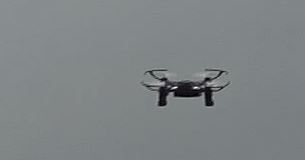
\includegraphics[width=4in]{dron.jpg}
	\caption{Fragment sekwencji testowej z widocznym dronem.}
	\label{fig:dron}
\end{figure}

%TODO Może w tym miejscu zdjęcia przykładowoe obiektu, zeby czytelnik wiedział mniej więcej o co chodzi. -zrobione.
Najpierw przeprowadzono test algorytmu śledzenia przez detekcję. Wykorzystano metodę detekcji polegającą na binaryzacji obrazu wejściowego i określeniu położenia obiektu jako środek masy obrazu wynikowego. Na rysunku \ref{fig:detekcja_test} przedstawiono przykładowy wynik testu.

\begin{figure}[h]
	\centering
	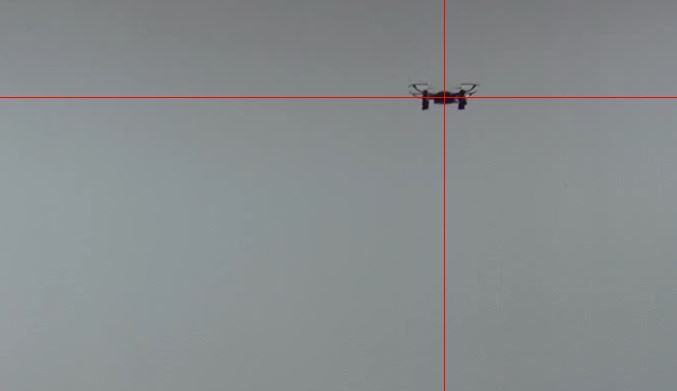
\includegraphics[width=4in]{detekcja_test.jpg}
	\caption{Wynik testu algorytmu śledzenia przez detekcję.}
	\label{fig:detekcja_test}
\end{figure}

Otrzymywano poprawne wyniki, jeśli śledzony obiekt był jedynym w kadrze i znacznie różnił się od tła. Użyto binaryzacji na podstawie jasności. Piksele, których jasność wynosiła poniżej \(50\), przyjmowano jako należące do obiektu. W efekcie algorytm przestawał działać, gdy w kadrze pojawiały się ciemne elementy (np. blat stołu), lub zmniejszone było oświetlenie.

Do oceny działania algorytmu Mean-shift wykorzystano funkcje napisane przez \textit{Sylvain Bernhardt}\cite{Bernhardt}. W testowanej metodzie zwiększona zostaje waga pikseli znajdujących się bliżej środka aktualnego okna. Na rysunku \ref{fig:meanshift_test} przedstawiono przykładowy wynik testu.

\begin{figure}[h]
	\centering
	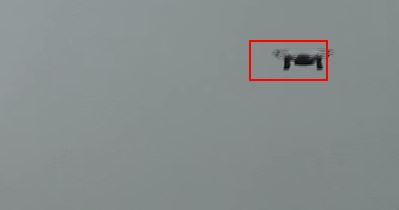
\includegraphics[width=4in]{meanshift_test.jpg}
	\caption{Wynik testu algorytmu Mean-shift.}
	\label{fig:meanshift_test}
\end{figure}

Czerwona ramka reprezentuje obecne okno. Algorytm gubił drona, kiedy ten wykonał szybkie ruchy. W pozostałych przypadkach algorytm poprawnie wskazywał położenie śledzonego obiektu.

Następnie sprawdzono działanie filtru cząsteczkowego. Użyto funkcji napisanych przez \textit{Sebastien Paris}\cite{Paris}. Testowany algorytm działał na obrazach w przestrzeni barw HSV. Wygenerowanych zostało 250 cząstek. Na rysunku \ref{fig:particle_test} przedstawiono przykładowy wynik testu.

\begin{figure}[h]
	\centering
	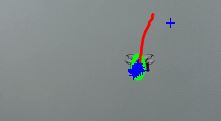
\includegraphics[width=4in]{particle_test.jpg}
	\caption{Wynik testu algorytmu filtru cząsteczkowego.}
	\label{fig:particle_test}
\end{figure}

Niebieski znaki '+' wskazują położenie cząsteczek. Algorytm działał dobrze, jeśli ruch obiektu był jednostajny. Dron był jednak gubiony, kiedy wykonywał ostre zwroty. Spowodowane jest to prawdopodobnie użytym modelem obiektu, który nie uwzględniał możliwości wykonywania takich manewrów.

Na końcu przetestowano algorytm KLT. Wykorzystano w tym celu wbudowane funkcje programu \textit{MATLAB}. Algorytm działa na obrazie w skali szarości. Do wykorzystanych funkcji przekazywano więc składową Y przestrzeni barw YUV. Na rysunku \ref{fig:klt_test} przedstawiono przykładowy wynik testu.

\begin{figure}[h]
	\centering
	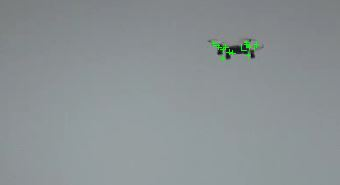
\includegraphics[width=4in]{klt_test.jpg}
	\caption{Wynik testu algorytmu KLT.}
	\label{fig:klt_test}
\end{figure}

Zielone znaki '+' wskazują położenia punktów charakterystycznych użytych do śledzenia obiektu. W trakcie testów stwierdzono, że duże ryzyko zgubienia obiektu pojawia się, gdy tło nie jest jednorodne (w otoczeniu występują punkty charakterystyczne).

Stwierdzono, że z zadaniem najlepiej poradził sobie algorytm KLT. 
Oprócz tego postanowiono zaimplementować prosty algorytm śledzenia przez detekcję do celów testowych.  
Przy jego użyciu badano pozycjonowanie serwomechanizmów w trakcie testowania i doboru nastaw regulatora. 
Został również przetestowany gotowy algorytm Mean-shift, aby sprawdzić jego działanie w platformie sprzętowej oraz ocenić skuteczność posiadanej implementacji.
%TODO powt. działanie. -zrobione.

%TODO W sumie to by się przyadło jakieś bardziej obszerne omówinie tych testów. Z przykładowoymi zdjęciami i opisaniem zachowania się poszczególnnych algorytmów. -zrobione. Mam nadzieję, że jest OK.